\chapter{Introduction}
\section{Internship Context}
This internship was conducted at CERMEP--Imagerie du Vivant in Lyon, France.
CERMEP is a research laboratory and imaging platform dedicated to preclinical and clinical in vivo imaging, including PET, MRI, and CT.
It also develops and produces radiopharmaceuticals for PET studies to support translational research in neuroscience, cardiology, and related fields.
The work took place in the PET--MR department, which operates a hybrid PET--MR scanner, conducts acquisition studies, and carries out methodological research.
The two datasets analyzed in this thesis were acquired at CERMEP using the clinical PET--MR system.
In this study, we also used in-house tools and software developed at CERMEP, including a PET simulation platform and the algorithm that formed the basis of this work.

\section{Positron Emission Tomography}
Positron Emission Tomography (PET) is an in vivo functional imaging technique widely used in clinical and research settings to monitor physiological and biochemical processes.
In PET, a biologically active molecule is labeled with a positron-emitting radioisotope, serving as a radiotracer, and then injected into the body.
As the radiotracer accumulates in target tissues, its radioactive decay produces positrons, which interact with electrons to emit pairs of gamma photons in nearly opposite directions.
These photons are detected by the PET scanner, and image reconstruction algorithms generate a three-dimensional representation of the tracer distribution.
This imaging modality allows for the investigation of metabolic changes, receptor binding, and other biochemical processes, providing invaluable information in oncology, neurology, cardiology, and other fields.

There are two main categories in PET image acquisition: static imaging and dynamic imaging.
Static PET involves acquiring a single scan after the radiotracer injection.
This single snapshot offers a powerful yet simplified view of tracer distribution.
The common quantification metric in static imaging is the Standardized Uptake Value (SUV), which normalizes tissue uptake by the injected dose and weight of the subject, allowing for a semi-quantitative comparison of tracer accumulation across different tissues or over time \cite{keyes1995suv}.
Due to its simplicity, static PET is widely used in clinical settings; however, it also has limitations.
Because it reflects only one time point, the SUV cannot capture the temporal dynamics of tracer uptake and clearance, and various physiological factors may influence its measurements, thereby reducing its accuracy.

Dynamic PET imaging provides a more comprehensive view of radiotracer kinetics by acquiring a series of images over a period ranging from a few minutes to more than an hour post-injection, depending on the tracer type.
Instead of a single snapshot, dynamic imaging produces time-activity curves (TAC) that illustrate how tracer concentration in each tissue changes throughout the scanning period.
This approach enables the measurement of physiological parameters such as the tracer rate of influx (\(K_i\)), volume of distribution (\(V_T\)), and binding potential (BP).

\section{Kinetic Modeling}
To quantify pharmacokinetic parameters, kinetic modeling is employed.
Compartmental modeling is the most popular and is considered the most accurate approach in kinetic modeling.
In compartmental modeling, the distribution and kinetics of a radiotracer are described by dividing the system into distinct compartments, each representing a pool of tracer that behaves uniformly.
Interactions between compartments can be unidirectional or bidirectional, meaning the tracer may either move in and out or only enter a compartment.
Various graphical models (e.g., the Logan \cite{logan1990graphical} and Patlak \cite{patlak1983graphical} methods), as well as classical compartmental model fitting approaches, are used to analyze tracer kinetics.

Figure~\ref{fig:2tcm} shows the two-tissue compartment model (2TCM), also known as the three-compartment model, in series mode.
This model comprises one tissue compartment for the free tracer, \(C_F(t)\), and another for the receptor-bound tracer, \(C_B(t)\), in addition to an external compartment representing the tracer concentration in the plasma or blood, denoted as the input function \(C_P(t)\).

The tracer kinetics are governed by a series of first-order differential equations, in which the exchange rates between the compartments are considered constant:
\begin{align}
	\frac{dC_F(t)}{dt} & = K_1 \, C_P(t) \;-\; \bigl(k_2 + k_3\bigr) C_F(t) \;+\; k_4 C_B(t) \,, \label{eq:2tcm-c1} \\[6pt]
	\frac{dC_B(t)}{dt} & = k_3 \, C_F(t) \;-\; k_4 \, C_B(t), \label{eq:2tcm-c2}
\end{align}
where \(K_1\), \(k_2\), \(k_3\), and \(k_4\) are the constant rate parameters.

\begin{figure}[b]
	\centering
	\begin{tikzpicture}[>=latex, thick,node distance=1.5cm]
		\node[cylinder, draw, shape border rotate=90, aspect=0.3, minimum height=2.5cm, minimum width=1.7cm, align=center, fill=red!80] (Cp) at (0,0) {$C_P$};
		\node[draw, rounded corners, minimum width=2.5cm, minimum height=2cm, align=center] (C1) at (4,0) {$C_F$};
		\node[draw, rounded corners, minimum width=2.5cm, minimum height=2cm, align=center] (C2) at (8,0) {$C_B$};


		\draw[->]
		([yshift=8pt]Cp.east) to[out=0, in=180]
		node[above] {\(K_1\)}
		([yshift=8pt]C1.west);

		\draw[->]
		([yshift=-8pt]C1.west) to[out=180, in=0]
		node[below] {\(k_2\)}
		([yshift=-8pt]Cp.east);

		\draw[->]
		([yshift=8pt]C1.east) to[out=0, in=180]
		node[above] {\(k_3\)}
		([yshift=8pt]C2.west);

		\draw[->, dashed, opacity=0.5]
		([yshift=-8pt]C2.west) to[out=180, in=0]
		node[below] {\(k_4 = 0\)}
		([yshift=-8pt]C1.east);

		% Draw yellow box in background
		\begin{pgfonlayer}{background}
			\coordinate (BoxTL) at ($(C1.north west)+(-0.3,0.3)$);
			\coordinate (BoxBR) at ($(C2.south east)+(0.3,-0.3)$);
			\coordinate (BoxTR) at ($(C2.north east)+(0.3,0.3)$);
			\draw[dashed, rounded corners, thick, fill=yellow!40] (BoxTL) rectangle (BoxBR);
		\end{pgfonlayer}

		% Blood label above Cp
		\node at ($(Cp.north)+(0,0.3)$) {\textbf{Blood}};

		\node at ($($(BoxTL)!0.5!(BoxTR)$)+(0,0.3)$) {\textbf{Tissue}};
		% \node[above] at ($($(C1.north west)+(-0.3,0.3)$)!0.5!($(C1.north east)+(-0.3,0.3)$)) {Tissue};
	\end{tikzpicture}%
	\caption{Schematic of the two-tissue compartment model (2TCM)}
	\label{fig:2tcm}
\end{figure}

The total radiotracer tissue kinetics measured by PET (the PET data), \(C_T(t)\), is given by
\begin{equation}
	C_T(t) \;=\; C_F(t) \;+\; C_B(t) \;+\; C_P(t).
\end{equation}

Thus, to solve this system of equations and to estimate \(K_1\), \(k_2\), and \(k_3\) parameters, we must fit the model using the measured PET TACs ($C_T$) and the input function ($C_P$).

For \fdg$\,$ quantification, the metabolic rate of glucose (\(\textrm{MR}_{\textrm{glu}}\)) is calculated as
\begin{equation}
	\textrm{MR}_{\textrm{glu}} \; (\textrm{\textmu mol/min/100g}) = \frac{[C]}{LC} \cdot \frac{K_1 \times k_3}{k_2 + k_3} \,.
\end{equation}
where \([C]\) denotes the glucose concentration, and \(LC\) is the lumped constant.

For \yohimbine\ quantification, we utilize the volume of distribution ($V_T$), which is the ratio of radiotracer concentration in the target tissue ($C_T$) to the plasma ($C_P$):
\[
	V_T = \frac{C_T}{C_P}
\]

Using the Logan plot method, this can be directly estimated from these two values, or it can be fitted with a compartment model.
In the latter case, $V_T$ can be calculated as
\[
	V_T = \frac{K_1}{k_2} (1+\frac{k_3}{k_4})
\]

\section{Input Function}

\subsection{Arterial Input Function}
The arterial input function (AIF) is considered the gold standard for obtaining the input function.
It is determined by inserting an arterial catheter into the patient and continuously drawing blood samples to measure the radiotracer concentration, thereby obtaining the blood activity curve used in the quantification model.
However, this procedure is invasive and can cause discomfort, potentially discouraging patients from undergoing future examinations.
Furthermore, this method is labor-intensive and requires trained personnel to manage both the subject and the measurement devices.

\subsection{Population-Based Input Function}
Population-Based Input Function (PBIF) is a method for replacing the subject-specific AIF with the average AIFs of a population of other subjects.
In practice, an average curve is derived from a representative cohort and then temporally aligned and scaled to the subject using one or more calibration points (e.g., early blood samples or image-derived peaks).
PBIF can reduce invasiveness and acquisition burden, but it may introduce bias if the cohort is not well matched to the subject or if calibration is suboptimal.

\subsection{Image-Derived Input Function}
The image-derived input function (IDIF) has been proposed as a non-invasive alternative for obtaining the input function.
IDIF techniques typically involve identifying vascular structures or regions with high blood pool activity within the imaging field and extracting the input function directly from the PET images.
For example, in whole-body, cardiac, or small-animal PET studies the aorta is visible in the Field of View (FOV) of the PET camera and is used as the source for IDIF.
In brain PET imaging, the Internal Carotid Arteries (ICA) are the largest vessels present in the FOV and have a diameter of approximately 5 mm, much smaller than the aorta.
Their smaller size makes IDIF more challenging due to partial volume effects (PVE).

\section{Partial Volume Effect}\label{sec:pve}
Partial Volume Effect (PVE) is the loss and mixing of signal that occurs when structures are small relative to the system’s spatial resolution, causing activity to “spill out” of small objects and “spill in” from neighbors.
In PET, this leads to systematic underestimation of arterial activity and contamination from surrounding tissue, especially for vessels like the ICA that have a similar size to the effective resolution of the PET camera (both around 5 mm).
In Figure~\ref{fig:pve}, this effect is illustrated by simulating the effect of PET's point spread function (PSF) as well as noise on a hot disk.
Correcting PVE is essential for accurate IDIF estimation and downstream kinetic modeling.

\begin{figure}[h]
	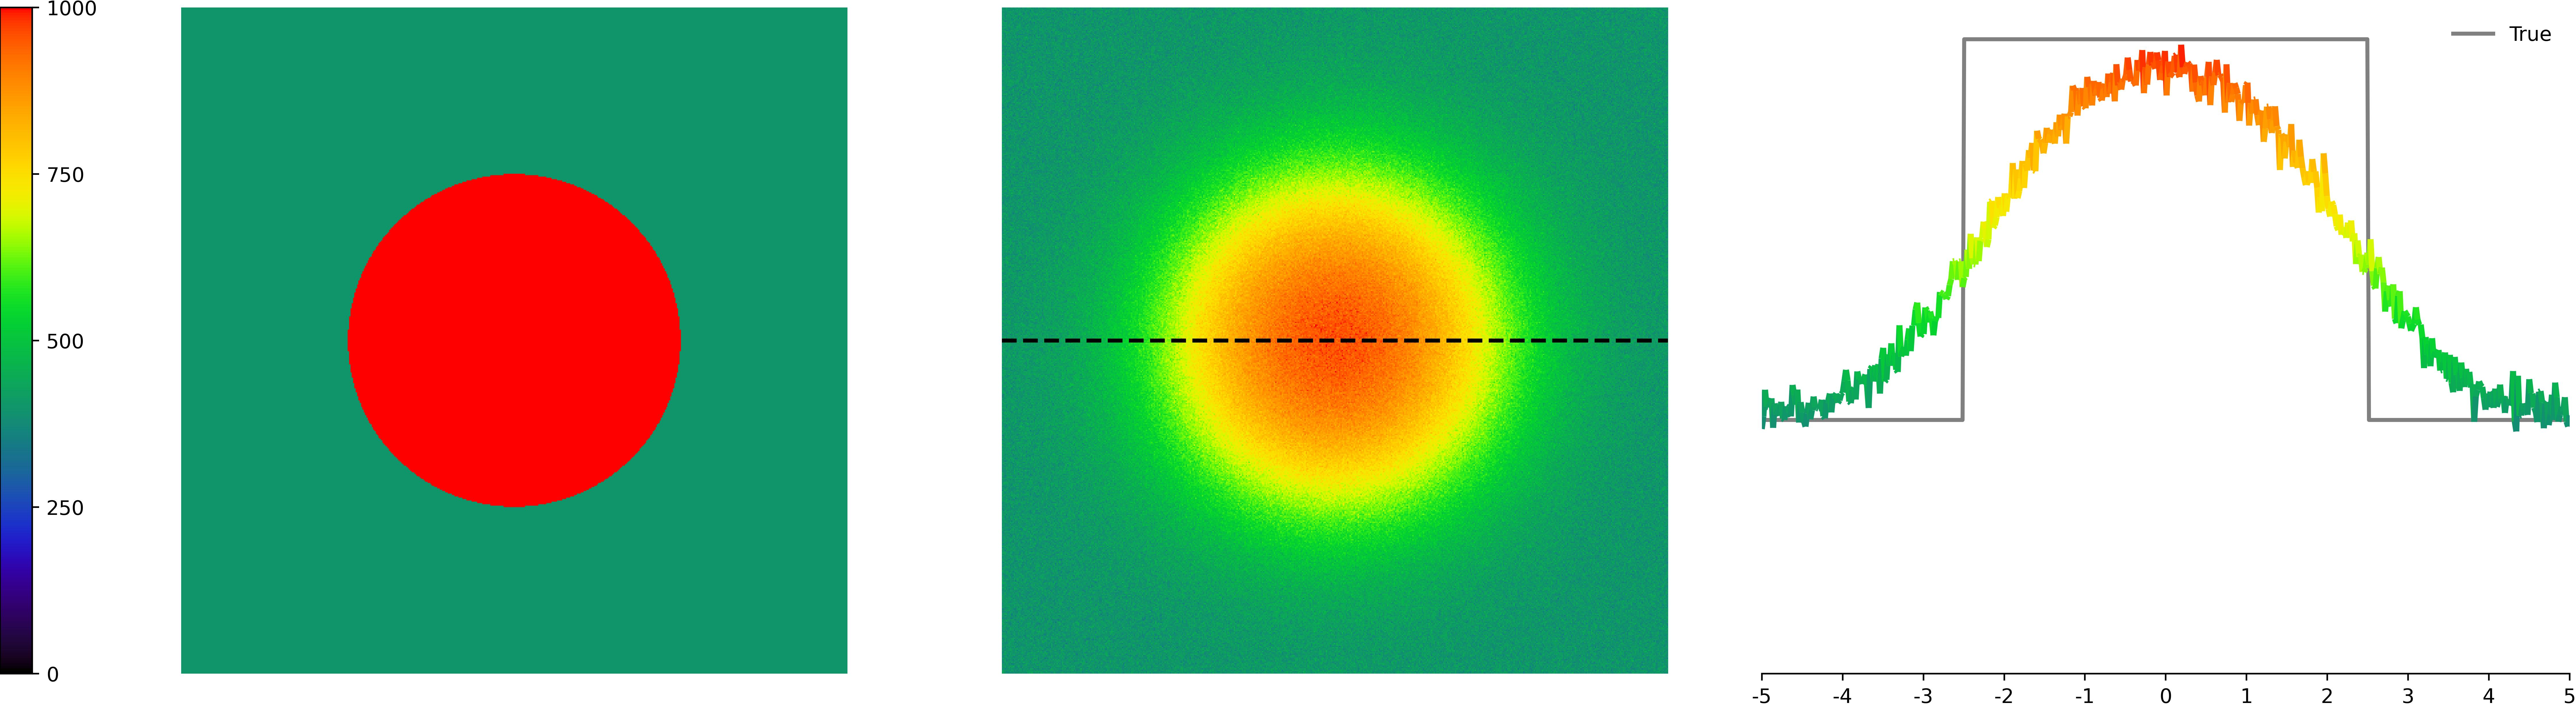
\includegraphics[width=\textwidth]{figures/pve.jpg}
	\caption{Partial Volume Effect shown on a uniform hot disk: left, the ground-truth disk; middle: the result of PET point spread function blurring and noise; right: intensity profile along the horizontal dashed-line compared to the ground truth (gray line), showing the spill-in and spill-out effects}
	\label{fig:pve}
\end{figure}
\section{Background}
Many methods have utilized the first few frames of the dynamic PET, when the tracer has not yet reached tissue and predominantly resides in the arteries, to obtain a mask of the carotids \cite{young2023image}.
These implementations range from fully manual approaches \cite{feng2015image}, to semi-automatic methods that use a few seed voxels for region growing or to initialize morphological operations \cite{dassanayake2022caliper,vestergaard2021validation}, and to fully automatic pipelines based on deep learning such as custom Convolutional Neural Networks (CNNs) \cite{ferrante2024physically,chen2025deep} and U-Net architectures \cite{chavan2024end}.

However, even with sophisticated approaches, ICA segmentation directly from PET suffers from strong PVE \cite{zanotti2011image,boellaard2004effects}.
With the emergence of hybrid PET/MRI systems, it has become feasible to acquire both functional and anatomical data simultaneously.
MRI provides high-resolution soft-tissue contrast, while PET captures metabolic activity.
For instance, time-of-flight MR angiography (TOF-MRA) delivers excellent arterial contrast.
Many studies have leveraged this to achieve accurate ICA segmentation using manual or semi-automatic procedures, typically relying on high-intensity thresholding and seeded or unseeded region growing \cite{feng2015image,sundar2019towards,sari2017estimation,jochimsen2016fully}.

Unlike T1-weighted MRI, TOF-MRA is not always included in research and clinical protocols.
Meanwhile, T1-weighted scans are routinely acquired for anatomical localization and image registration, among other purposes, which makes them a practical source for arterial segmentation when TOF-MRA is not part of the protocol.
In this context, \citeauthor{rahman2024deep} \cite{rahman2024deep} proposed a deep learning model that infers the ICA directly from T1-weighted images.

As noted above, even with a high-resolution anatomical arterial mask, PVE remains and must be corrected.
Partial Volume Correction (PVC) methods estimate spill-in and spill-out coefficients between the ICA and surrounding tissue.
Recovery Coefficients (RC) are commonly used, obtained by scanning cylindrical phantoms of various diameters and matching the ICA diameter to the closest phantom \cite{dassanayake2022caliper,lyoo2014image}.
The Geometric Transfer Matrix (GTM) method generalizes this by estimating regional spillover based on volume geometry and an explicit point spread function (PSF) model \cite{rousset1998correction}.
However, these linear mixing models do not account for additional effects such as time-varying noise or motion, and they typically treat the problem as a fixed linear unmixing without propagating uncertainty, which can limit recovery.

More advanced approaches include model-based matrix factorization that jointly estimates the input function and tissue activity \cite{fang2022image}; non–deep-learning strategies that infer the blood curve without explicit vessel segmentation—such as factor analysis / cluster-IDIF, population-based input functions, and optimization-derived input functions \cite{simoncic2015image,lyoo2014image,dias2022clinical}; and deep learning \cite{kawauchi2023convolutional}.

In this work, we propose a fully automatic pipeline for extracting the ICA mask from TOF-MRA.
We then employ a Bayesian framework that couples GTM-based mixing with priors on the input function and tissue kinetics, explicitly modeling noise to improve IDIF estimation \cite{irace2021bayesian} aiming to eliminate the need for invasive arterial blood sampling in dynamic PET imaging.

